% flashcards-title: Vector components on a Cartesian grid
% flashcards-desc: Vector A begins at the origin and ends four grid units right and three grid units up. Dashed projection lines connect its head to the x- and y-axes.
\documentclass[border=5mm]{standalone}
\def\pgfsysdriver{pgfsys-dvisvgm.def}
\usepackage{tikz}
\usetikzlibrary{arrows.meta,calc,patterns.meta,positioning}
\renewcommand{\familydefault}{\sfdefault}

\definecolor{fcInk}{HTML}{1C1C1E}
\definecolor{fcMuted}{HTML}{68686D}
\definecolor{fcGuide}{HTML}{C9C9CE}
\definecolor{fcGold}{HTML}{D7A313}
\definecolor{fcGoldSoft}{HTML}{F8E8AE}

\tikzset{
  fc canvas/.style={fill=white, rounded corners=2.5mm},
  fc vector/.style={
    draw=fcGold,
    line width=1.35mm,
    line cap=round,
    -{Stealth[length=4.1mm,width=3.25mm]}
  },
  fc vector secondary/.style={
    draw=fcInk,
    line width=1.15mm,
    line cap=round,
    dash pattern=on 4.1mm off 2.6mm,
    -{Stealth[length=3.9mm,width=3.1mm]}
  },
  fc resultant/.style={
    draw=fcMuted,
    line width=1.55mm,
    line cap=round,
    -{Stealth[length=4.6mm,width=3.6mm]}
  },
  fc axis/.style={
    draw=fcInk,
    line width=.72mm,
    -{Stealth[length=3.1mm,width=2.5mm]}
  },
  fc guide/.style={
    draw=fcMuted,
    line width=.55mm,
    dash pattern=on 2.3mm off 1.8mm
  },
  fc construction/.style={draw=fcGuide, line width=.32mm},
  fc endpoint/.style={circle, fill=fcInk, inner sep=1.45mm},
  fc label/.style={font=\bfseries\large, text=fcInk},
  fc small label/.style={font=\small, text=fcMuted},
  fc caption/.style={font=\bfseries\small, text=fcMuted}
}

\begin{document}
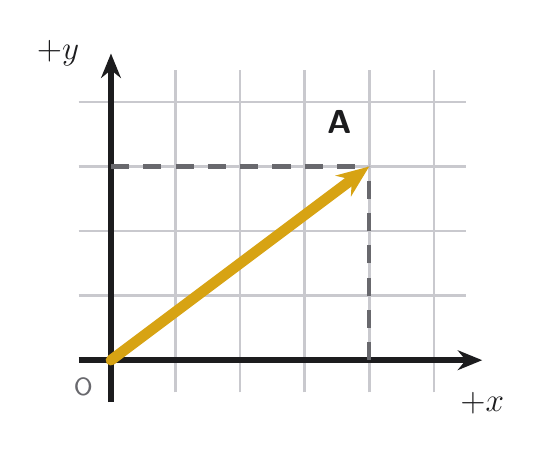
\begin{tikzpicture}[x=.82cm,y=.82cm]
  \path[fc canvas] (-1.05,-1.15) rectangle (6.15,5.15);
  \draw[fc construction, step=1] (-.5,-.5) grid (5.5,4.5);
  \draw[fc axis] (-.5,0) -- (5.75,0) node[fc label, below=2.5mm] {$+x$};
  \draw[fc axis] (0,-.65) -- (0,4.75) node[fc label, left=2.5mm] {$+y$};
  \node[fc small label, below left=1.5mm] at (0,0) {O};

  \draw[fc guide] (4,0) -- (4,3);
  \draw[fc guide] (0,3) -- (4,3);
  \draw[fc vector] (0,0) -- (4,3);
  \node[fc label, above left=3mm and 1mm] at (4,3) {A};
\end{tikzpicture}
\end{document}
